\documentclass{article}[18pt]
\usepackage[utf8]{inputenc}
\usepackage[margin=0.7in]{geometry}
\usepackage{parselines} 
\usepackage{amsmath}
\usepackage{titlesec}
\usepackage{pgfplots}
\usepackage{graphicx}
\usepackage[english]{babel}
\usepackage{fancyhdr}
\usepackage{gensymb}
\usepackage{relsize}
\pgfplotsset{width=10cm,compat=1.9}

\titlespacing\section{0pt}{14pt plus 4pt minus 2pt}{0pt plus 2pt minus 2pt}
\newlength\tindent
\setlength{\tindent}{\parindent}
\setlength{\parindent}{0pt}
\renewcommand{\indent}{\hspace*{\tindent}}

\pagestyle{fancy}
\fancyhf{}
\rhead{Sam Robbins 13SE}
\lhead{A Level Maths - FP2}
\rfoot{Page \thepage}


\begin{document}
\begin{center}
\underline{\huge First Order Differential Equations}
\end{center}
\section{Families of curves}
General solutions with a constant of integration C will give rise to a family of curves.\\
\\
If given boundary conditions we can find specific solutions.
\subsection{Example}
Find the solution to:\\
\\
$\dfrac{dy}{dx}=2$\\
\\
$y=2x+c$\\
\\

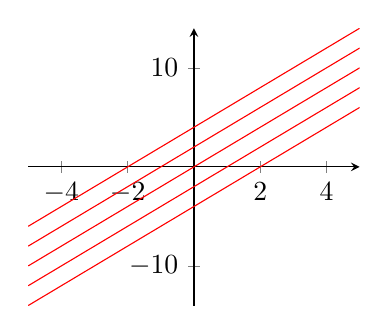
\begin{tikzpicture}
\begin{axis}[axis lines=middle,scale=0.5]
\addplot[color=red]{2*x};
\addplot[color=red]{2*x+2};
\addplot[color=red]{2*x+4};
\addplot[color=red]{2*x-2};
\addplot[color=red]{2*x-4};
\end{axis}
\end{tikzpicture}


\end{document}